\documentclass[a4paper]{article}

%\usepackage{times}
\usepackage{epsfig}
\usepackage{graphicx}
\usepackage{amsmath}
\usepackage{amsthm}
\usepackage{amssymb}
\usepackage{color}
\usepackage{subcaption}
\usepackage[left = 30mm, right = 30mm, bottom = 30mm, top = 30mm]{geometry}
\usepackage{hyperref}
\hypersetup{
	colorlinks=true,
	linkcolor=red,
	filecolor=magenta,      
	urlcolor=blue,
}

% load package with ``framed'' and ``numbered'' option.
%\usepackage[framed,numbered,autolinebreaks,useliterate]{mcode}

% something NOT relevant to the usage of the package.
\setlength{\parindent}{0pt}
\setlength{\parskip}{18pt}

%\usepackage[latin1]{inputenc} 
%\usepackage[T1]{fontenc} 

\usepackage{listings} 
\lstset{% 
   language=Matlab, 
   basicstyle=\small\ttfamily, 
   frame=single,
} 

\newcommand*\diff{\mathop{}\!\mathrm{d}}

\setlength{\fboxsep}{0pt}

\title{Pattern Recognition\\Exercise 2}
\author{Mario Kaufmann \\ Ramona Imhof \\ Jakob Sch\"arer \\ Adrian W\"alchli \\ Jan Liechti}

\begin{document}

\maketitle

\section{SVM}

\section{MLP}

\subsection{Implementation with standard MATLAB tools}

\subsection{Implementation with NN Toolbox}
As an alternative approach, we used the Neural Network toolbox from {MATLAB} to implement the {MLP}.
We used cross-validation to find the optimal number of neurons in the hidden layer as well as the optimal learning rate.
We adapted a grid search on the following search space:
\begin{itemize}
	\item Layer size: 50, 60, 70, ..., 150
	\item Eight learning rates on the interval $[0.001, 0.05]$
\end{itemize}
We found the optimal parameters are 140 neurons and 0.001 for the learning rate.
On the full training set, the runtime for the parameter search is about 25 minutes.
We save the performance for the best network and show it in figure~\ref{fig:perf-vs-epoch-toolbox}.
The classification accuracy on the test set with these parameters is \textbf{96.2736} percent.
\begin{figure}[tb]
	\centering
	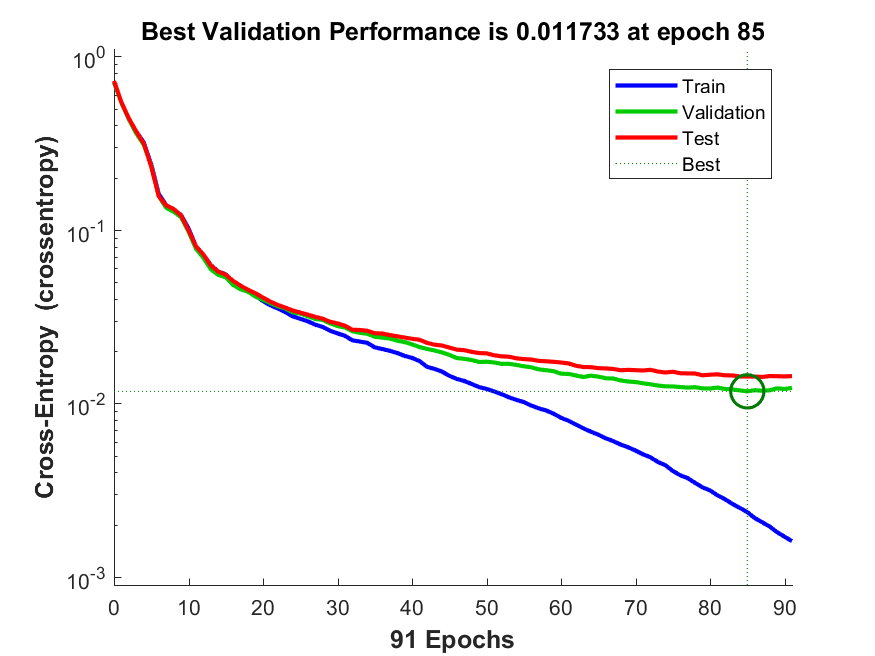
\includegraphics[width=12cm]{{images/mlp-versionB-toolbox/Performance-vs-epochs-hidden=140-LR=0.001000}.png}
	\caption{Cross-entropy error vs. epochs. 
			 The test set in this figure is not the same as the test set we use for the final evaluation.
			 These are the three splits to verify the performance during training. 
			 We abort after 6 validation checks (when the performance does not improve anymore).}
	\label{fig:perf-vs-epoch-toolbox}
\end{figure}


\end{document}